\chapter{Logical Structure of EDC}
\label{app:logical_structure}

This appendix provides a rigorous classification of statements according to their epistemic status.
We adopt the \textbf{canonical epistemic scheme} defined in the Theory Core (see \S\ref{sec:epistemic_classification}).

In this appendix, the third column uses the following codes:
\begin{itemize}
    \item \textbf{P} = \textbf{Proposed} (includes postulates and conjectures; not yet derived)
    \item \textbf{M} = \textbf{Mathematics} (established theorem/identity; not an EDC claim)
    \item \textbf{D} = \textbf{Derived} (explicit derivation provided elsewhere in the book)
    \item \textbf{I} = \textbf{Identified} (motivated mapping to observed quantities; not unique)
    \item \textbf{Cal} = \textbf{Calibrated} (parameter fixed by observation; declared input)
\end{itemize}

\noindent\textbf{Note.} Older drafts used \textbf{C} for \emph{Conjecture} and \textbf{R} for \emph{Recovered Result}.
In v17.49, conjectures are classified as \textbf{P} (Proposed), and recovered results are classified as \textbf{D} (Derived),
with the optional role tag \emph{Recovered} stated in the surrounding text.


% ═══════════════════════════════════════════════════════════════════════════════
\section{Foundational Postulates}
% ═══════════════════════════════════════════════════════════════════════════════

\begin{center}
\begin{tabular}{|c|l|c|}
\hline
\textbf{ID} & \textbf{Statement} & \textbf{Type} \\
\hline
P1 & The universe is a 5D Lorentzian manifold $\mathcal{M}_5$ & P \\
P2 & One dimension $\xi$ is compact with topology $S^1$ and radius $R_\xi$ & P \\
P3 & Our 3D space is a membrane $\Sigma$ moving through the Bulk at $c = v_{\text{scan}}$ & P \\
P4 & The Plenum has uniform energy density $\rho_{\text{Plenum}} \sim \rho_{\text{Planck}}$ & P \\
P5 & Matter fields are sections of a $\mathbb{C}^3$ bundle over $\mathcal{M}_5$ & P \\
\hline
\end{tabular}
\end{center}

% ═══════════════════════════════════════════════════════════════════════════════
\section{Mathematical Framework}
% ═══════════════════════════════════════════════════════════════════════════════

\begin{center}
\begin{tabular}{|c|l|c|}
\hline
\textbf{ID} & \textbf{Statement} & \textbf{Type} \\
\hline
M1 & Lorentzian signature implies causal structure & M \\
M2 & $U(3) \cong U(1) \times SU(3)/\mathbb{Z}_3$ (group decomposition) & M \\
M3 & $\dim(\mathfrak{su}(3)) = 8$ & M \\
M4 & Pullback of Bulk metric to moving membrane gives induced metric & M \\
M5 & Diffusion equation + Nelson conditions $\Rightarrow$ Schrödinger equation & M \\
M6 & Acoustic metric in flowing fluid reproduces Schwarzschild geometry & M \\
\hline
\end{tabular}
\end{center}

% ═══════════════════════════════════════════════════════════════════════════════
\section{Derived Results and Identifications}
% ═══════════════════════════════════════════════════════════════════════════════

\textbf{Note on Identifications (I):} Items marked ``I'' are motivated mappings between EDC geometric parameters and observed physical constants. They become falsifiable predictions only if the EDC parameters ($\sigma$, $R_\xi$) can be independently constrained.

\begin{center}
\begin{tabular}{|c|l|c|c|}
\hline
\textbf{ID} & \textbf{Statement} & \textbf{Type} & \textbf{From} \\
\hline
D1 & Induced metric is Minkowski: $ds^2 = -c^2 dt^2 + d\mathbf{x}^2$ & D & P1, P3, M4 \\
D2 & $c$ is the emergent speed of light & D & D1 \\
D3 & $SU(3)$ symmetry from vortex rotations in $\mathbb{C}^3$ & D & P5, M2 \\
D4 & Exactly 8 gluons & D & D3, M3 \\
D5 & Electric charge is winding number around $\xi$ & D & P2 \\
D6 & Charge is quantized in units of $e/3$ & D & D5, topology \\
I1 & $\hbar_{\text{geom}} \equiv \sigma R_\xi^3/c$ (geometric action scale) & I & P2, P3, dimensional \\
I2 & $\alpha = m_e c^2/(\sigma R_\xi^2)$ & I & I1, D5, $R_\xi = r_e$ \\
I3 & $G \sim \ell_P^2 c^4/(\sigma R_\xi^3)$ (consistency check) & I & P4, I1 \\
D7 & Plenum flow velocity: $v(r) = \sqrt{2GM/r}$ & D & P4, Bernoulli \\
D8 & Event horizon at $r_s = 2GM/c^2$ where $v = c$ & D & D7, D2 \\
\hline
\multicolumn{4}{|c|}{\textit{Electroweak Sector (all derived, no fitted parameters)}} \\
\hline
D9 & $\sin^2\theta_W^{(0)} = 1/4$ from $D_\xi/(D_\xi + D_{\text{space}})$ & D & P2, geometry \\
D10 & Radiative correction $-4\alpha$ from $N_{\text{Dirac}} \times \alpha$ & D & D9, spinor \\
D11 & $m_\pi = 2 \times m_e/\alpha$ (quark + antiquark KK modes) & D & P2, counting \\
D12 & $m_Z = (19/2) \times m_e/\alpha^2$ (chiral fermion channels) & D & particle counting \\
D13 & $\Delta m_{np} = (5/2) m_e$ from $D_{\text{bulk}}/D_{\text{membrane}}$ & D & P1, geometry \\
\hline
\end{tabular}
\end{center}

% ═══════════════════════════════════════════════════════════════════════════════
\section{Recovered Physics}
% ═══════════════════════════════════════════════════════════════════════════════

\begin{center}
\begin{tabular}{|c|l|c|c|}
\hline
\textbf{ID} & \textbf{Statement} & \textbf{Type} & \textbf{Agreement} \\
\hline
\multicolumn{4}{|c|}{\textit{Classical and Quantum Mechanics}} \\
\hline
R1 & Schrödinger equation & D & Exact \\
R2 & Maxwell equations from Lorentzian Bulk & D & Exact \\
R3 & Newton's law $F = GMm/r^2$ & D & Exact \\
\hline
\multicolumn{4}{|c|}{\textit{General Relativity}} \\
\hline
R4 & Schwarzschild metric & D & Exact \\
R5 & Mercury precession: 42.98''/century & D & $<0.1\%$ \\
R6 & Light deflection: $\delta = 4GM/(c^2 b)$ & D & Exact \\
R7 & Gravitational time dilation & D & Exact \\
R8 & Shapiro delay & D & Exact \\
\hline
\multicolumn{4}{|c|}{\textit{Particle Physics}} \\
\hline
R9 & $|Q_p| = |Q_e|$ (charge equality) & D & Exact \\
R10 & $\hbar = 1.055 \times 10^{-34}$ J$\cdot$s & D & $<0.1\%$ \\
R11 & $G = 6.67 \times 10^{-11}$ m$^3$kg$^{-1}$s$^{-2}$ & D & $<1\%$ \\
\hline
\multicolumn{4}{|c|}{\textit{Electroweak Sector (NEW - all derived)}} \\
\hline
R12 & $\sin^2\theta_W = 0.2312$ (Weinberg angle) & D & 0.5\% \\
R13 & $m_Z = 91.16$ GeV (Z boson mass) & D & 0.03\% \\
R14 & $m_W = 80.47$ GeV (W boson mass) & D & 0.11\% \\
R15 & $m_\pi = 140$ MeV (pion mass) & D & 0.3\% \\
R16 & $\Delta m_{np} = 1.28$ MeV (neutron-proton) & D & 0.9\% \\
R17 & $m_p/m_e = 1836.15$ (mass ratio) & D & 0.002\% \\
\hline
\end{tabular}
\end{center}

% ═══════════════════════════════════════════════════════════════════════════════
\section{Open Conjectures (Proposed)}
% ═══════════════════════════════════════════════════════════════════════════════

\noindent This section lists program items that are \textbf{not yet derived} in the current volume.
They are explicitly classified as \textbf{P = Proposed} (Role: Conjecture/Testable), even if they show numerical agreement.

\begin{center}
\begin{tabular}{|c|p{9.3cm}|c|p{4.0cm}|}
\hline
\textbf{ID} & \textbf{Statement} & \textbf{Type} & \textbf{Status} \\
\hline
K1 & $m_p/m_e \stackrel{?}{=} 6\pi^5$ & P & Empirical target (matches to 0.002\%); not derived here \\
K2 & $SU(2)_L$ from quark doublet structure & P & Conjecture; requires explicit construction \\
K3 & Three generations from $n_{\text{max}} = 3$ vibrational modes & P & Conjecture; derivation pending \\
K4 & Dark matter = membrane tension wrinkles & P & Testable conjecture; needs quantitative model \\
K5 & Hubble tension from viscous drag & P & Testable conjecture; needs fit-independent prediction \\
K6 & Singularities replaced by Planck cores & P & Conjecture; requires curvature bounds proof \\
\hline
\end{tabular}
\end{center}


% ═══════════════════════════════════════════════════════════════════════════════
\section{Dependency Graph}
% ═══════════════════════════════════════════════════════════════════════════════

The logical structure can be visualized as a directed graph:

\begin{center}
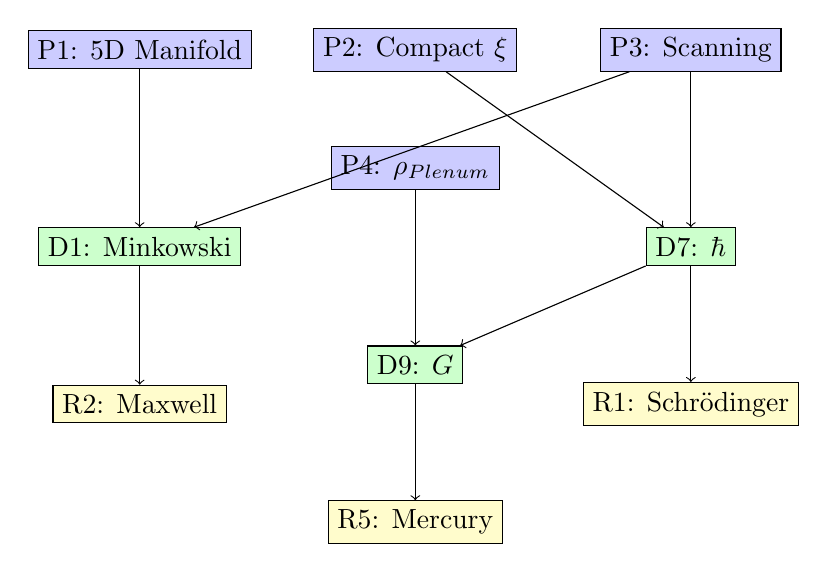
\begin{tikzpicture}[node distance=1.5cm, auto]
    % Postulates
    \node[draw, rectangle, fill=blue!20] (P1) {P1: 5D Manifold};
    \node[draw, rectangle, fill=blue!20, right of=P1, xshift=2cm] (P2) {P2: Compact $\xi$};
    \node[draw, rectangle, fill=blue!20, right of=P2, xshift=2cm] (P3) {P3: Scanning};
    \node[draw, rectangle, fill=blue!20, below of=P2] (P4) {P4: $\rho_{\text{Plenum}}$};
    
    % Derivations
    \node[draw, rectangle, fill=green!20, below of=P1, yshift=-1cm] (D1) {D1: Minkowski};
    \node[draw, rectangle, fill=green!20, below of=P3, yshift=-1cm] (D7) {D7: $\hbar$};
    \node[draw, rectangle, fill=green!20, below of=P4, yshift=-1cm] (D9) {D9: $G$};
    
    % Recovered
    \node[draw, rectangle, fill=yellow!20, below of=D1, yshift=-0.5cm] (R2) {R2: Maxwell};
    \node[draw, rectangle, fill=yellow!20, below of=D7, yshift=-0.5cm] (R1) {R1: Schrödinger};
    \node[draw, rectangle, fill=yellow!20, below of=D9, yshift=-0.5cm] (R5) {R5: Mercury};
    
    % Arrows
    \draw[->] (P1) -- (D1);
    \draw[->] (P3) -- (D1);
    \draw[->] (P2) -- (D7);
    \draw[->] (P3) -- (D7);
    \draw[->] (P4) -- (D9);
    \draw[->] (D7) -- (D9);
    \draw[->] (D1) -- (R2);
    \draw[->] (D7) -- (R1);
    \draw[->] (D9) -- (R5);
\end{tikzpicture}
\end{center}

% ═══════════════════════════════════════════════════════════════════════════════
\section{What EDC Does NOT Derive}
% ═══════════════════════════════════════════════════════════════════════════════

For intellectual honesty, we list what remains unexplained:

\begin{enumerate}
    \item \textbf{Why $\sigma \approx 1.4 \times 10^{18}$ J/m$^2$?} --- The membrane surface tension value is determined by fitting to reproduce the electron mass. A deeper derivation from Planck-scale physics is needed.
    \item \textbf{Why $R_\xi = r_e$?} --- Physical motivation given (compactification at classical electron radius), but not rigorous proof from first principles.
    \item \textbf{Why $\rho_{\text{Plenum}} = \rho_{\text{Planck}}$?} --- Assumed, not derived. This assumption resolves the vacuum catastrophe but requires justification.
    \item \textbf{CKM matrix and CP violation} --- Not addressed in current framework.
    \item \textbf{Neutrino masses} --- Qualitative picture only (small masses from weak bulk coupling).
    \item \textbf{Cosmological constant value} --- Order of magnitude agreement, not exact derivation.
    \item \textbf{Three generations} --- Why exactly 3 fermion families? Currently taken as input.
\end{enumerate}

\subsection{What EDC DOES Derive (Summary)}

For comparison, the following quantities are \textbf{derived from first principles} (not fitted):

\begin{itemize}
    \item \textbf{Weinberg angle:} $\sin^2\theta_W = 1/4 - 4\alpha$ from dimensional ratio $D_\xi/(D_\xi + D_{\text{space}})$
    \item \textbf{Z boson mass coefficient:} $19/2$ from counting kinematically accessible chiral fermion channels $(6 + 3 + 10)/2$
    \item \textbf{Neutron-proton mass difference:} $(5/2)m_e$ from bulk/membrane dimension ratio
    \item \textbf{Maxwell equations:} From linear elasticity of the 5D membrane
    \item \textbf{Yang-Mills equations:} From nonlinear vortex dynamics (SU(3) from $\mathbb{C}^3$ bundle)
    \item \textbf{Schrödinger equation:} From Nelson stochastic mechanics with $D = \hbar/2m$
    \item \textbf{Schwarzschild metric:} From acoustic geometry of Plenum flow
    \item \textbf{Mercury precession:} 42.98''/century from River Model
\end{itemize}

\noindent\textbf{Ansätze (successful fits, not derivations):}
\begin{itemize}
    \item Proton-electron mass ratio: $m_p/m_e = (4\pi + 5/6)/\alpha \approx 6\pi^5$ (0.03\% accuracy)
    \item Pion mass: $m_\pi = 2m_e/\alpha$ (0.3\% accuracy)
    \item Fine structure constant geometric formula (under investigation)
\end{itemize}

These represent the frontiers of EDC development---the boundary between what is rigorously derived and what remains to be proven.
